\documentclass[english]{article}
\usepackage[T1]{fontenc}
%\usepackage[latin9]{inputenc}
%\usepackage{geometry}
%\geometry{verbose,tmargin=1in,bmargin=1in,lmargin=1in,rmargin=1in}
\usepackage{amsmath}
\usepackage{amssymb}
\usepackage{setspace}
\usepackage[utf8]{inputenc}
\usepackage{graphicx}
\usepackage{float}
\usepackage{adjustbox}
\usepackage{gensymb}
\usepackage{amssymb}
\usepackage{array}
\usepackage{ragged2e}
\usepackage{lipsum}
\onehalfspacing
\usepackage{babel}
\usepackage{tikz}
\usepackage{ctable}
\usepackage{booktabs}
\usepackage{graphicx}
\usepackage{caption}
\usepackage{placeins}
\usepackage{todonotes}
\usepackage{subcaption}
\usepackage[font=footnotesize,labelformat=simple]{subcaption}
\usepackage[T1]{fontenc}
\usepackage{pdflscape}

\begin{document}

\title{Informality in LAC: Heterogeneity and Disappointing Progress}
\maketitle
\begin{abstract}
    This descriptive paper uses household and employment surveys from the Latin America and the Caribbean region to paint a more complete picture of the different aspects of informality. We start by discussing alternative informality measures at the regional and cross country level. We then show that there has been progress on increasing the share of dependent workers who contribute to social security but that the productive structure of the economies in the region has remained mostly unchanged. We argue that this is mainly coming from the focus of governments policies on facilitating the registration of low productivity workers, therefore subsidizing low productivity firms. To make this point we use two approaches: a qualitative approach based on the analysis of policies that have been identified as successful in reducing informality. Second, we use a simple decomposition on different formalization margins to show that the formalization process in the region has been dominated by workers transitioning to formal status in the same type of firm. This means that the progress made in formalizing workers has happened mainly through increasing coverage of workers in small firms. 
\end{abstract}
\section{Introduction}
\begin{itemize}
    \item Motivation: Informality is a pervasive problem in the region despite many attempts to curtail it. The discussion around informality has been     \item What is informality? 
    
    The mainstream measure of informality comes from the ILO and is interested in following and comparing phenomena that are related but different. 
    \begin{itemize}
        \item Low productivity
        \item Unprotected workers
        \item Unlawful employment
    \end{itemize}
   This paper is divided in two sections the first section looks under the hood of the mainstream informality definition, studies the evolution of alternative measures trying to characterize different segments of informality, document the progress made in reducing informality in the region in the last two decades and their different margins. The second section goes over a summary of the reforms that have been implemented in the region with the goal of reducing informality. 
\end{itemize}
\section{Complexity of Informality}
\begin{itemize}
    \item Mention the history of the term and related literature: Harris Todaro 1970, De Soto, Perryet. al. Ulyssea 2017
 
    \item The mainstream definition of informality comes from the ILO (include the matrix showing the definition of informality). Check the documents coming out of the statistical meeting where they define informality and try to get the concerns behind. 
    \item Include a disaggregation of the different types of ILO informality ( prior: social security explains most of the informal)
       \item International organization have produce many flagship reports on informality : incluir OECD, WB 2021 shadow economy, ILO , IDB, etc. 
       \item the regional discussion has constantly portrayed informality as a public enemy.  
    \item In the next section we look separately at the different components of informality and relate each component with the main policy concern that explains...
\end{itemize}

\section{Labor Market Structure of the Average LAC Country}

\begin{figure}[H]
                \justifying
                \caption{Informality rate vs GDP percapita PPP}  
                \centerline{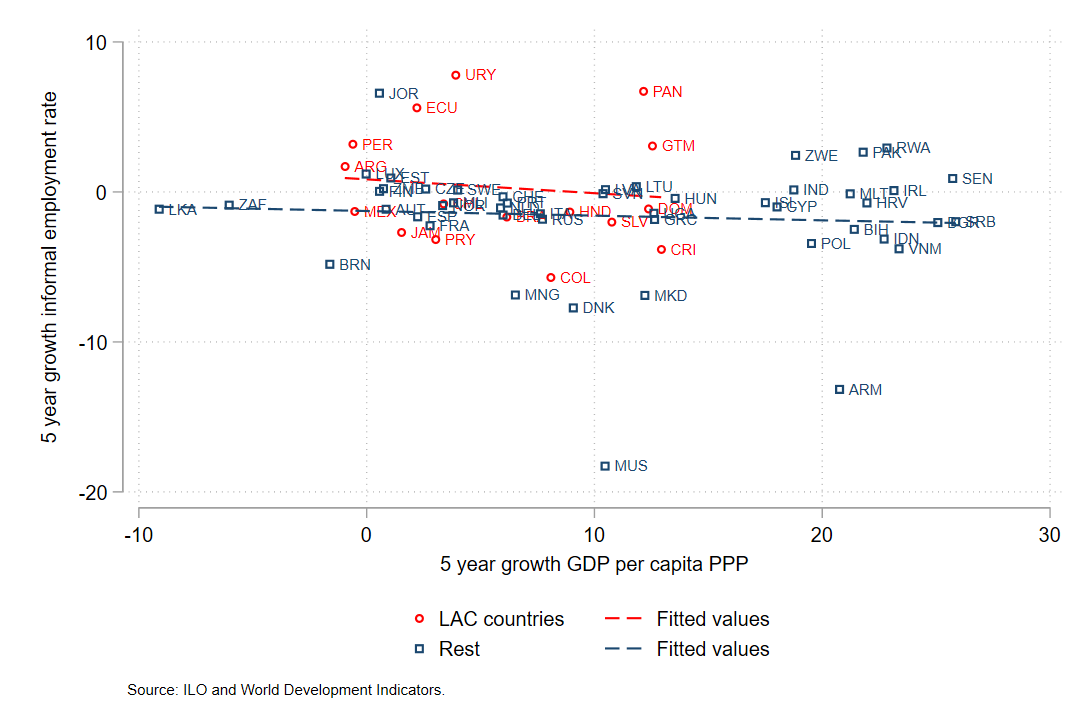
\includegraphics[scale=.3]{latex/figures/Evolution/Lastyear_growth.png}}
                \label{fig:info_gdp}
                \footnotesize{Source: ILO and World Development indicators.}
             \end{figure}

\begin{itemize}
    \item Alternative informality definitions
             \begin{figure}[H]
                \justifying
                \caption{Alternative informality definitions 2022}  
                \centerline{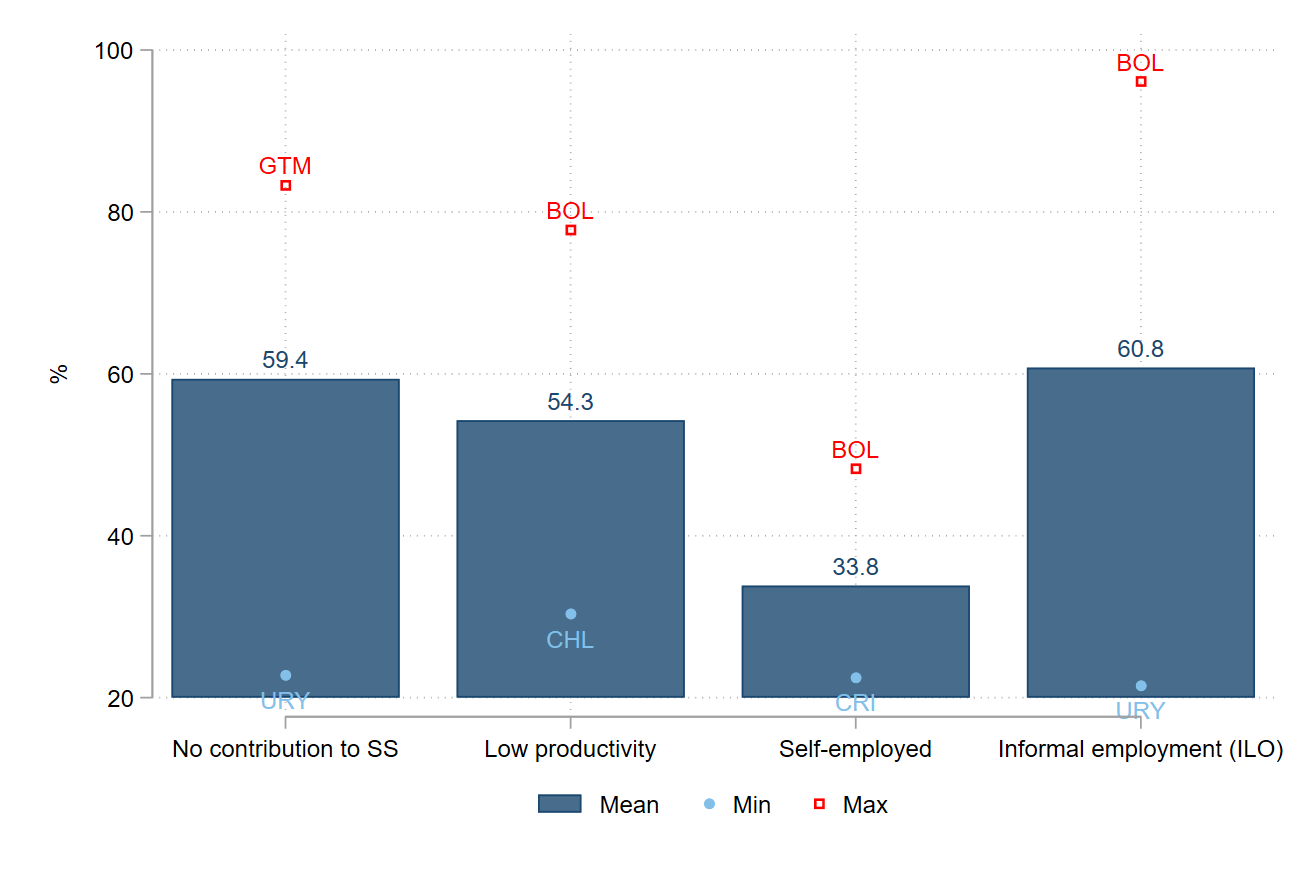
\includegraphics[scale=.3]{latex/figures/Snapshot/Alternative informality definitions_2022.png}}
                \label{fig:info_definitions}
                \footnotesize{Source: Household Surveys-SEDLAC and ILO.}
                \footnotesize{Note: Each bar is a simple average of country level data in 2022. Countries included in the sample: Argentina, Bolivia, Brazil, Chile, Colombia, Costa Rica, Dominican Republic, Ecuador, El Salvador, Guatemala, Honduras, Mexico, Panama, Peru, Paraguay and Uruguay. For countries without information for 2022 in SEDLAC we use the last available year: Bolivia 2021; Guatemala 2014; Honduras 2019 and Panama 2021. Note: Productive definition includes these groups of workers: salaried worker in small private firm, self-employed with less than completed tertiary education, unpaid workers and employer in small private firms.}
             \end{figure}

              \begin{figure}[H]
                \justifying
                \caption{Alternative informality definitions evolution}  
                \centerline{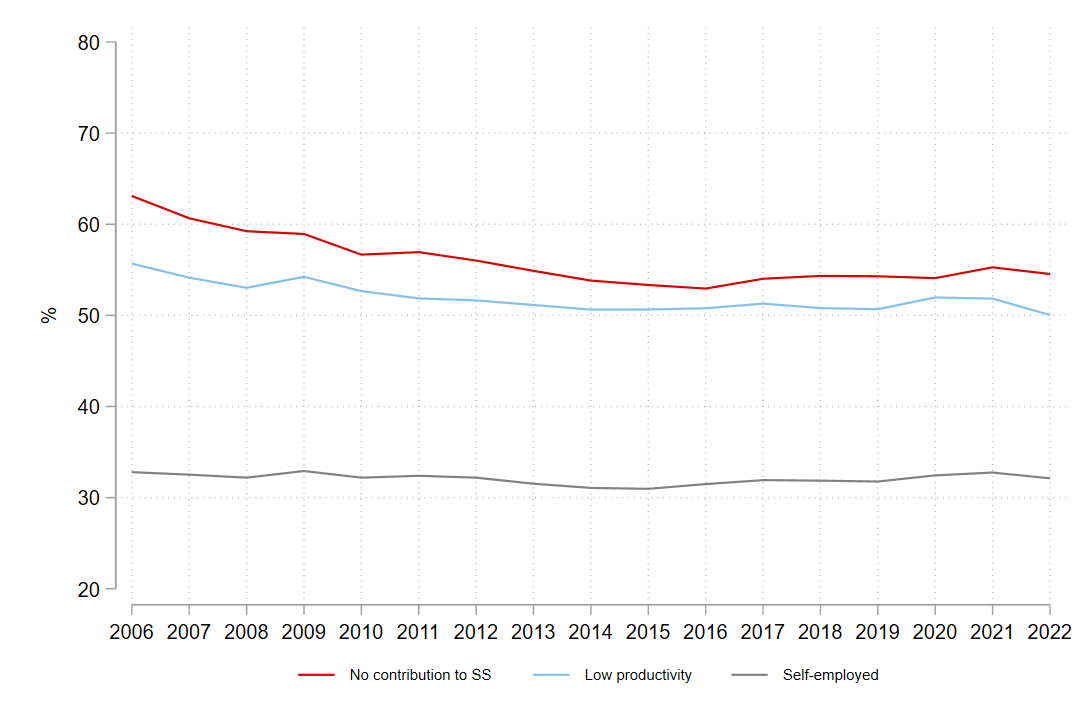
\includegraphics[scale=.3]{latex/figures/Evolution/LAC_informalitydefs_v2.png}}
                \label{fig:info_defevolution}
                \footnotesize{Source: Household Surveys-SEDLAC and ILO.}
                \footnotesize{Note: Each line represents a simple average of country-level data. The countries included are: Argentina, Bolivia, Brazil, Chile, Colombia, Costa Rica, Dominican Republic, Ecuador, El Salvador, Guatemala, Honduras, Mexico, Panama, Peru, Paraguay and Uruguay. Colombia start in the series since 2008 due to is GEIH's first year. Please note that Mexico experienced a survey change in 2014, and results from both surveys are included in this figure.}
             \end{figure}

             \begin{figure}[H]
                \justifying
                \caption{Self-employed by education level}  
                \centerline{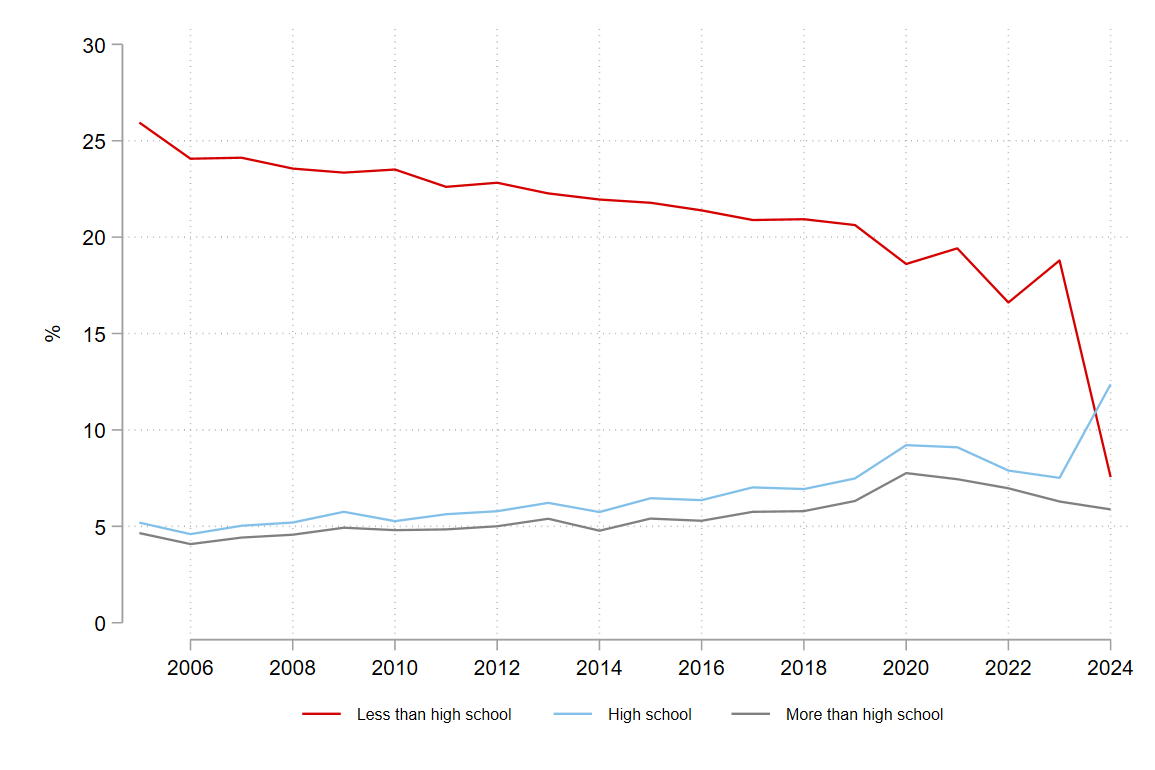
\includegraphics[scale=.3]{latex/figures/Evolution/LAC_selfemployment_educlevel.png}}
                \label{fig:se_evolution}
                \footnotesize{Source: Household Surveys-SEDLAC.}
                \footnotesize{Note: Each line is a simple average of country level data.}
             \end{figure}

             \begin{figure}[H]
                \justifying
                \caption{Self-employed workers who contributes to SS evolution by education level}  
                \centerline{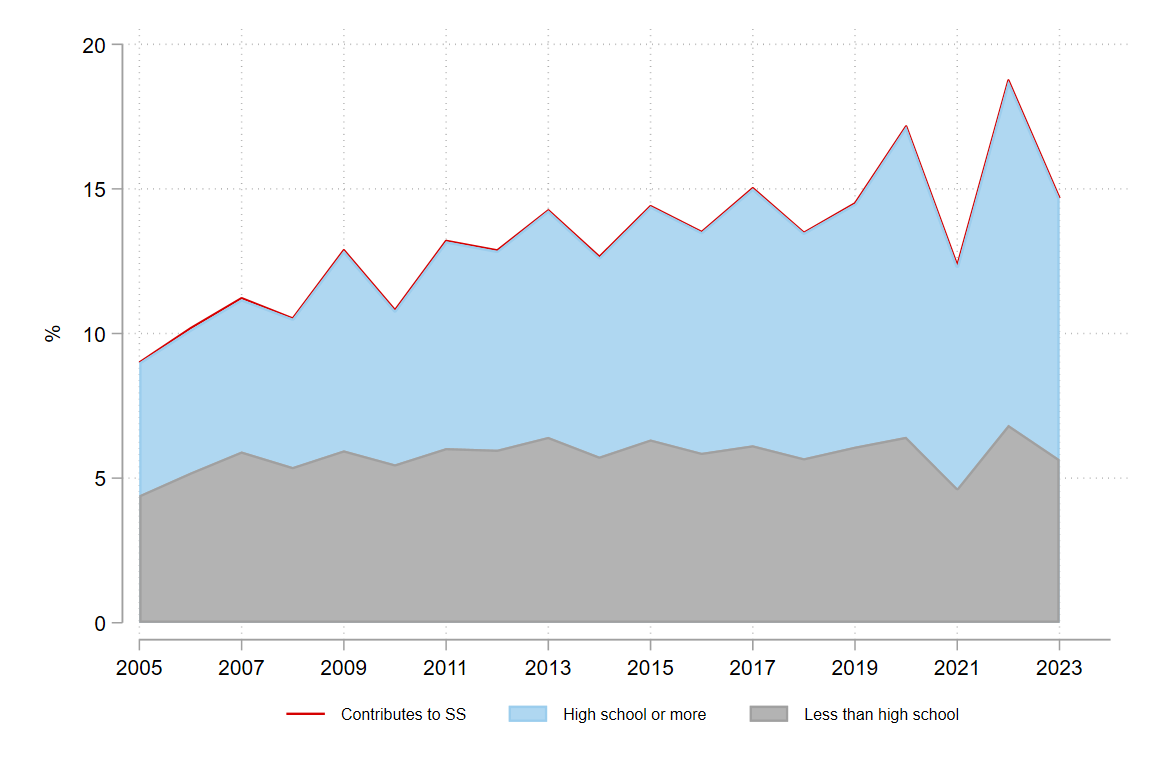
\includegraphics[scale=.3]{latex/figures/Evolution/LAC_selfemployment_educ.png}}
                \label{fig:se_evolution}
                \footnotesize{Source: Household Surveys-SEDLAC.}
                \footnotesize{Note: Each line is a simple average of country level data. Note:Uruguay is excluded from 2020.}
             \end{figure}
            
        \item Structure of the labor market 
    
        Figures \ref{fig:labmarket1} and \ref{fig:labmarket2} shows the structure of the labor market for the average latin american country. 
        
            \begin{figure}[H]
                \justifying
                  \caption{Demographic profile and structure of labor market}
                \begin{subfigure}{.9\textwidth}
                      \centering
                      \subcaption{Demographic}
                      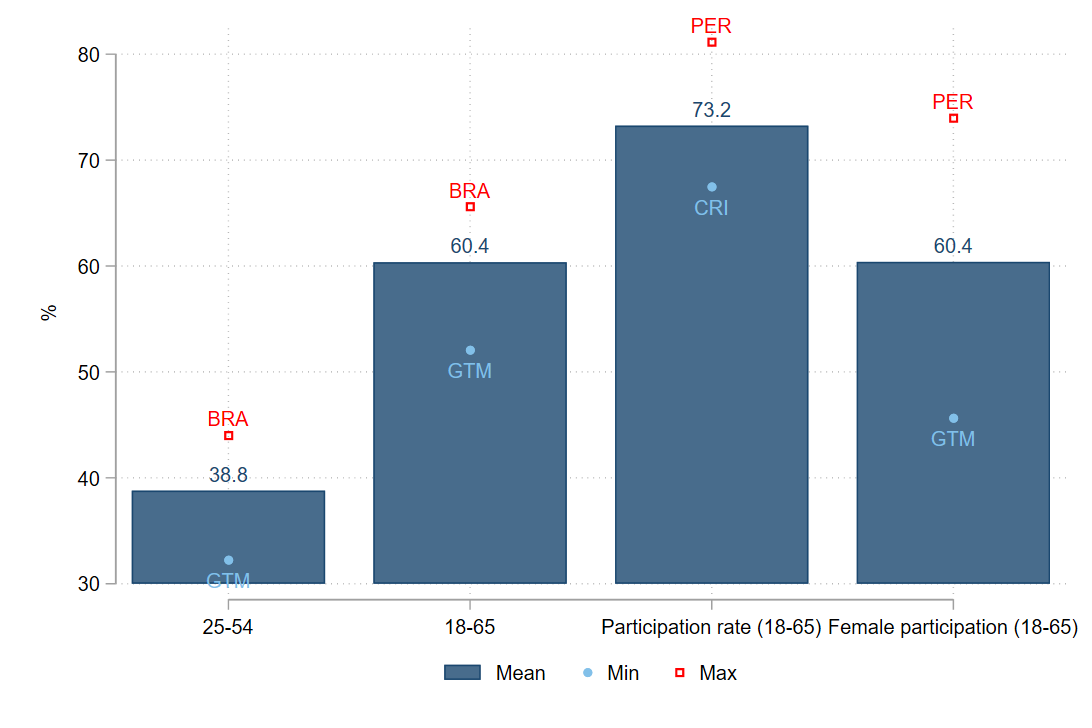
\includegraphics[width=1\linewidth]{latex/figures/Snapshot/Structure of labor market_a.png}
                      \label{fig:labmarket1}
                \end{subfigure}
        
                \begin{subfigure}{.9\textwidth}
                      \centering
                      \subcaption{Labor market}
                      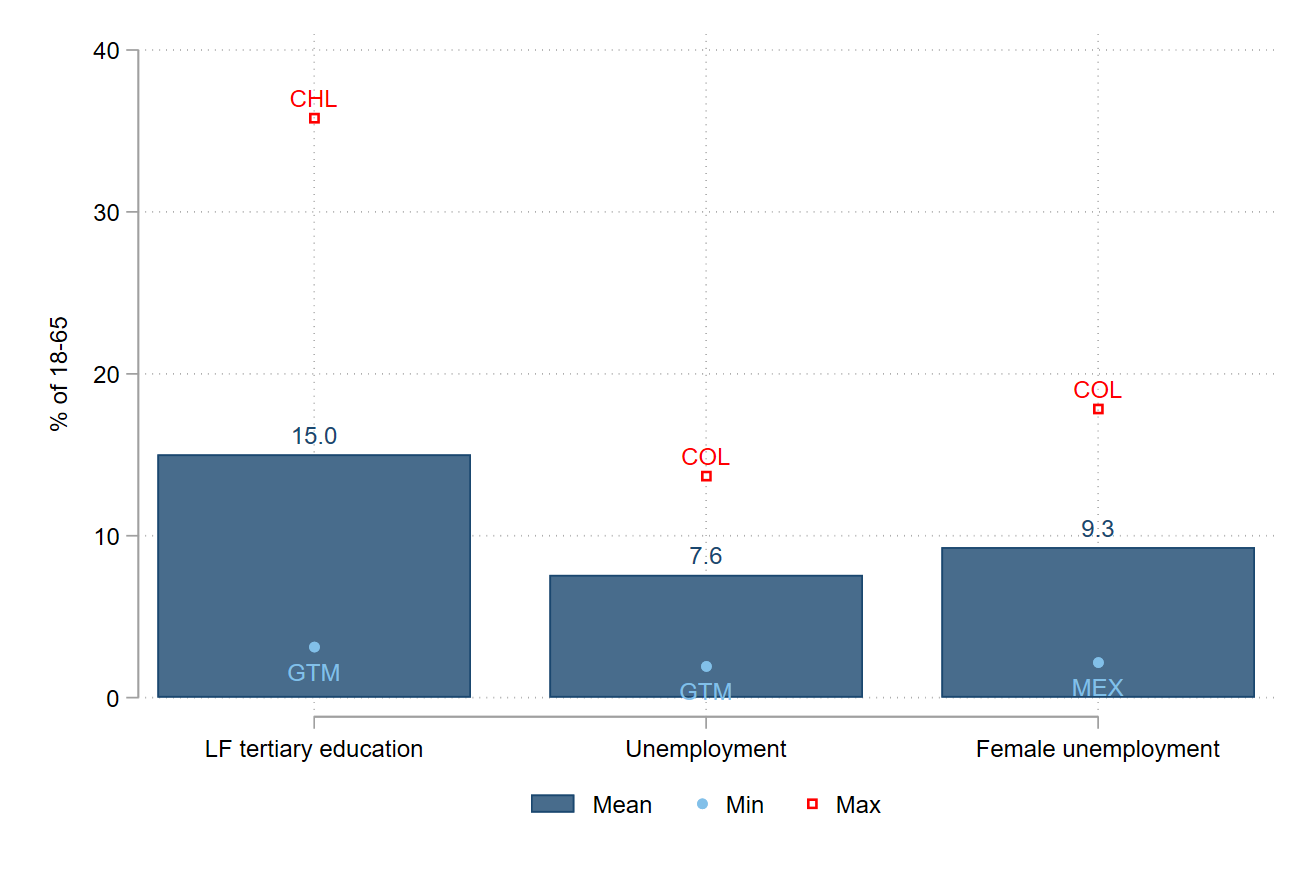
\includegraphics[width=1\linewidth]{latex/figures/Snapshot/Structure of labor market_b.png}
                      \label{fig:labmarket2}
                \end{subfigure}
        
                 \footnotesize{Source: Household Surveys-SEDLAC.}
                \footnotesize{Note: Each bar is a simple average of country level data in 2022. Countries included in the sample: Argentina, Bolivia, Brazil, Chile, Colombia, Costa Rica, Dominican Republic, Ecuador, El Salvador, Guatemala, Honduras, Mexico, Panama, Peru, Paraguay and Uruguay. For countries without information for 2022 in SEDLAC we use the last available year: Bolivia 2021; Guatemala 2014; Honduras 2019 and Panama 2021. Panel a: bar one and two are defined as percentage of the population. Also, "Participation rate" and "Female participation" are define as part of the labor force defined for people between 18 and 65 years old. Panel b: "LF tertiary education" corresponds to people in the workforce who have completed tertiary education.}
        
            \end{figure}
      
        \item Structure of Employment
        
            \begin{figure}[H]
                \justifying
                \caption{Structure of employment}     
                \centerline{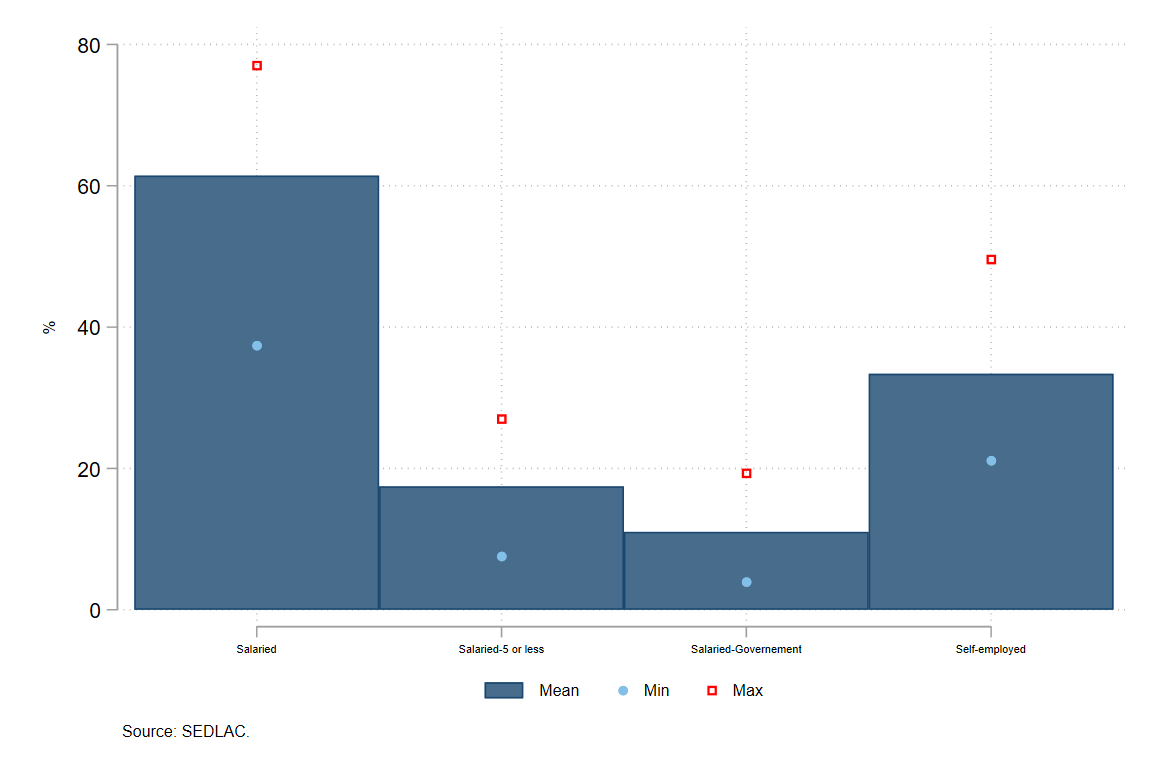
\includegraphics[scale=.3]{latex/figures/Snapshot/Structure of employment.png}
                \label{fig:employment}}
                \footnotesize{Source: Household Surveys-SEDLAC.}
                \footnotesize{Note: Each bar is a simple average of country level data in 2022. Countries included in the sample: Argentina, Bolivia, Brazil, Chile, Colombia, Costa Rica, Dominican Republic, Ecuador, El Salvador, Guatemala, Honduras, Mexico, Panama, Peru, Paraguay and Uruguay. For countries without information for 2022 in SEDLAC we use the last available year: Bolivia 2021; Guatemala 2014; Honduras 2019 and Panama 2021. The "non-salaried" category corresponds to unpaid workers such as family or cooperative workers.}
            \end{figure}
    
    
            \begin{figure}[H]
                \centering
                \caption{Structure of salaried and self-employed workers} 
                \centerline{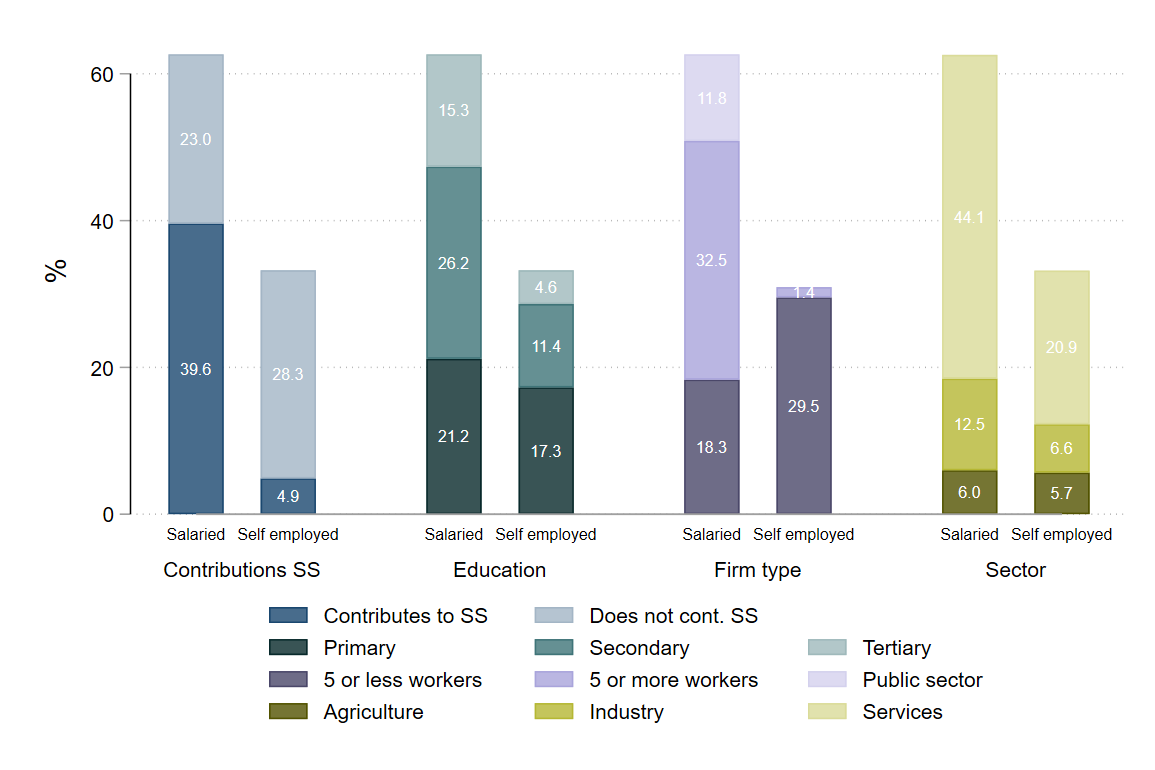
\includegraphics[scale=.3]{latex/figures/Snapshot/Snapshot salaried and self-employed.png}
                \label{fig:employmentbars}}
                \justifying
                \footnotesize{Source: Household Surveys-SEDLAC.}
                \footnotesize{Note: Each bar is a simple average of country level data in 2022. Countries included in the sample: Argentina, Bolivia, Brazil, Chile, Colombia, Costa Rica, Dominican Republic, Ecuador, El Salvador, Guatemala, Honduras, Mexico, Panama, Peru, Paraguay and Uruguay. For countries without information for 2022 in SEDLAC we use the last available year: Bolivia 2021; Guatemala 2014; Honduras 2019 and Panama 2021. Argentina only has information on contributions to social security for salaried workers, we are assuming all self-employed workers do not contribute.}
    
            \end{figure}
             
    
            
        \item Structure of Employment II - Sector and Contribution to SS
    
            \begin{figure}[H]
                \justifying
                \caption{Structure of employment by sector}     
                \centerline{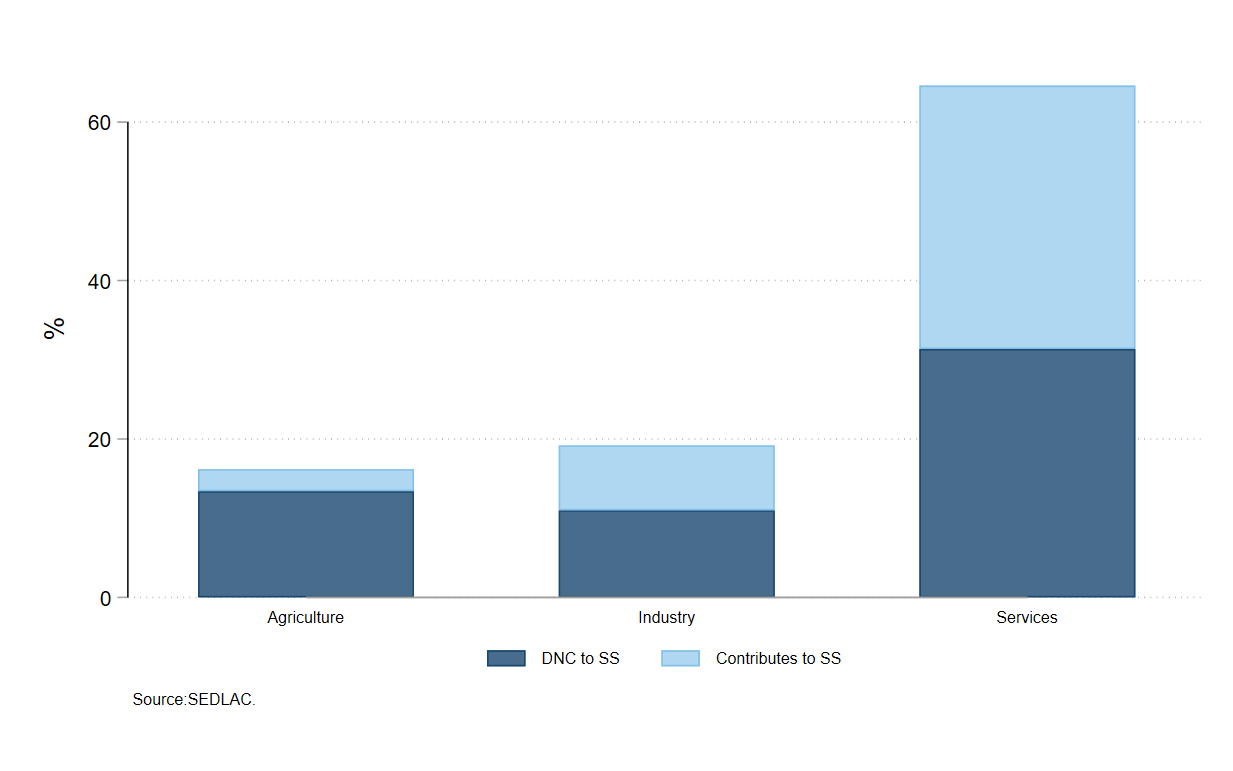
\includegraphics[scale=.3]{latex/figures/Snapshot/Structure of employment and sector.png}
                \label{fig:sector}}
               \footnotesize{Source: Household Surveys-SEDLAC.}
                \footnotesize{Note: Each bar is a simple average of country level data in 2022. Countries included in the sample: Argentina, Bolivia, Brazil, Chile, Colombia, Costa Rica, Dominican Republic, Ecuador, El Salvador, Guatemala, Honduras, Mexico, Panama, Peru, Paraguay and Uruguay. For countries without information for 2022 in SEDLAC we use the last available year: Bolivia 2021; Guatemala 2014; Honduras 2019 and Panama 2021. Argentina is excluded from this figure because the household survey is urban.}
            \end{figure}
    
            
        \item Employment by Firm Size
            \begin{figure}[H]
                    \justifying
                    \caption{Structure of private employment by firm size}     
                    \centerline{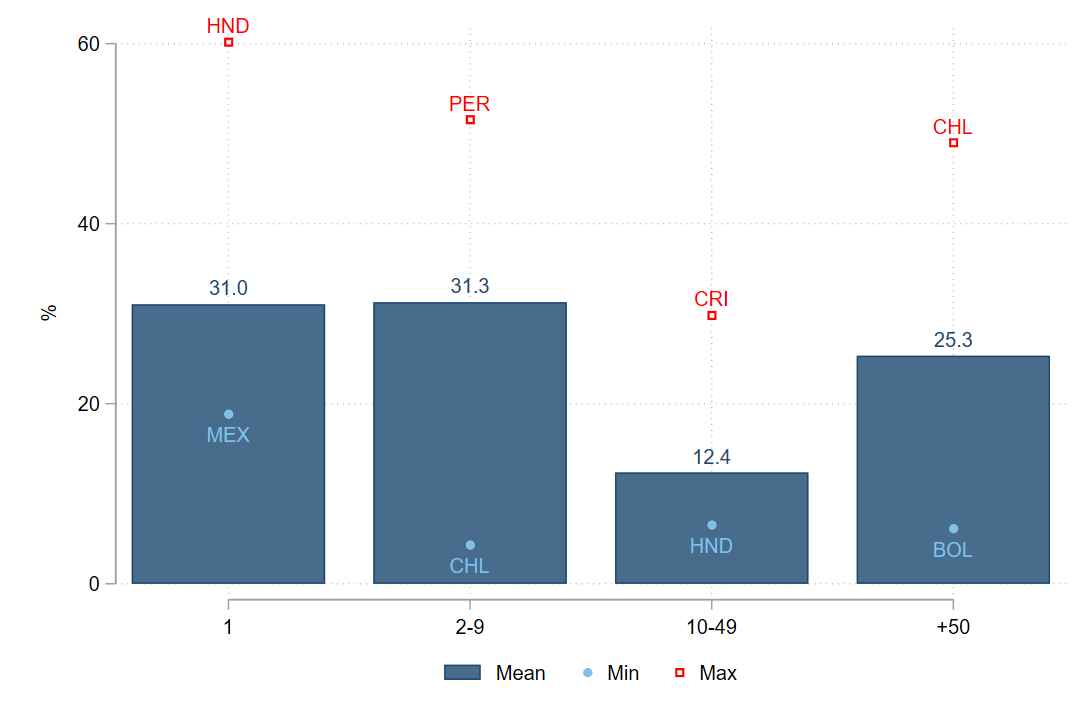
\includegraphics[scale=.3]{latex/figures/Snapshot/Structure of employment by firm size.png}
                    \label{fig:firmsize}}
                    \footnotesize{Source: Household Surveys-SEDLAC.}
                    \footnotesize{Note: Each bar is a simple average of country level data in 2022. Countries included in the sample: Argentina, Bolivia, Brazil, Chile, Colombia, Costa Rica, Dominican Republic, Ecuador, El Salvador, Guatemala, Honduras, Mexico, Panama, Peru, Paraguay and Uruguay. For countries without information for 2022 in SEDLAC we use the last available year: Bolivia 2021; Guatemala 2014; Honduras 2019 and Panama 2021. We exclude Argentina, Dominican Republic and Guatemala, because of missing information in firm size variable.}
            \end{figure}
    
    
            
        \item Social security contributions
                    \begin{figure}[H]
                    \justifying
                    \caption{Share of Workers Who Do Not Contribute to Social Security by Selected Characteristics}
                    \centerline{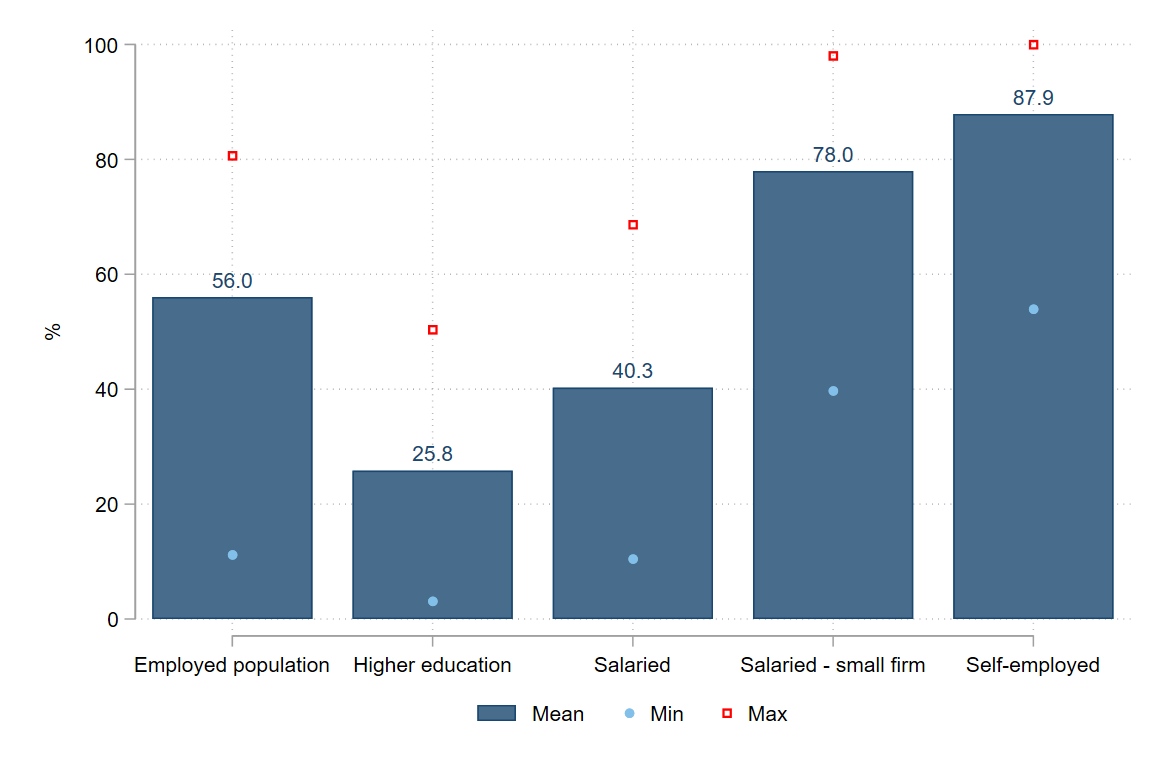
\includegraphics[scale=.3]{latex/figures/Snapshot/Social security contributions.png}
                    \label{fig:SScontributions}}
                    \footnotesize{Source: Household Surveys-SEDLAC.}
                    \footnotesize{Note: Each bar is a simple average of country level data in 2022. Countries included in the sample: Argentina, Bolivia, Brazil, Chile, Colombia, Costa Rica, Dominican Republic, Ecuador, El Salvador, Guatemala, Honduras, Mexico, Panama, Peru, Paraguay and Uruguay. For countries without information for 2022 in SEDLAC we use the last available year: Bolivia 2021; Guatemala 2014; Honduras 2019 and Panama 2021.
                    \textbf{The groups are not exclusive.} "Tertiary education" corresponds to people in the workforce who have completed tertiary level of education. "Salaried-Small firm" are salaried employees that work in a firm of 5 or less workers.}
            \end{figure}
    
    
        \item Life cycle- self employment and salaried informal
             \begin{figure}[H]
                        \justifying
                        \caption{Average Age profile in a LAC country}     
                        \centerline{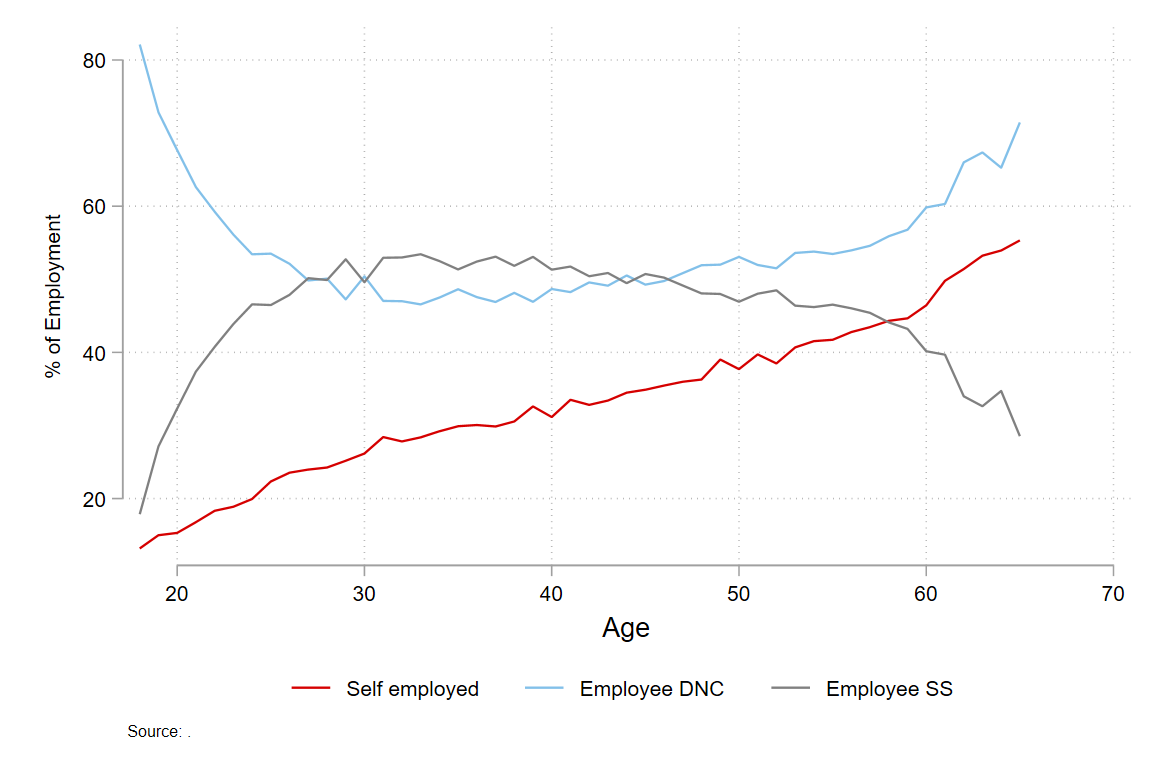
\includegraphics[scale=.3]{latex/figures/Snapshot/age_profile.png}
                        \label{fig:age_pro}}
                        \footnotesize{Source: Household Surveys-SEDLAC.}
                        \footnotesize{Note: Each line is a simple average of country level data. Country level data is computed weighting by total workers. Countries included in the sample: Argentina, Bolivia, Brazil, Chile, Colombia, Costa Rica, Dominican Republic, Ecuador, El Salvador, Guatemala, Honduras, Mexico, Panama, Peru, Paraguay and Uruguay. Data corresponds to 2022. For countries without information for 2022 in SEDLAC we use the last available year: Bolivia 2021; Guatemala 2014; Honduras 2019 and Panama 2021.}
             \end{figure}
\end{itemize}
        
     
\section{Dynamics: last 20 years}  

\subsection{Cross country figures}
\subsubsection{Household}
\begin{figure}[H]
    \justifying
     \caption{Snapshot of LAC’s household contribution status}     \centerline{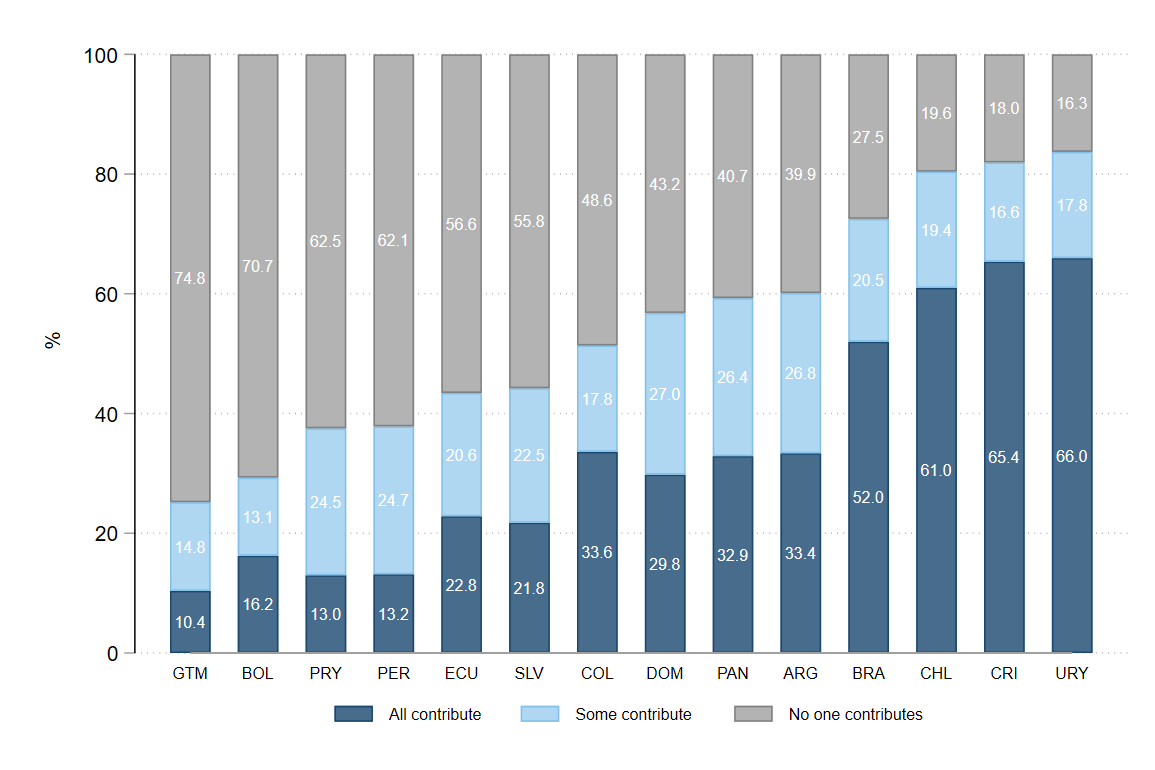
\includegraphics[scale=.3]{latex/figures/Household/snapshot_household.png}
    \label{fig:Householdlastyear}}
    \footnotesize{Source: Household Surveys-SEDLAC.}
    \footnotesize{Note: Each bar is a weighted average of each country, weighting by total workers in 2022. For countries without information for 2022 in SEDLAC we use the last available year: Bolivia 2021; Guatemala 2014; Honduras 2019 and Panama 2021.}
    \footnotesize{Note: The figure reports the household contribution status to social security of households with at least one member works. All contribute: corresponds to the percentage of households where all workers contribute to SS. Some contribute: corresponds to the percentage of households where some workers contribute to SS but not all. No one contributes: corresponds to the percentage of households where no workers contributes to SS.}
\end{figure}

\begin{figure}[H]
    \justifying
     \caption{Snapshot of LAC’s household employment condition for 2005-2022}     
     \centerline{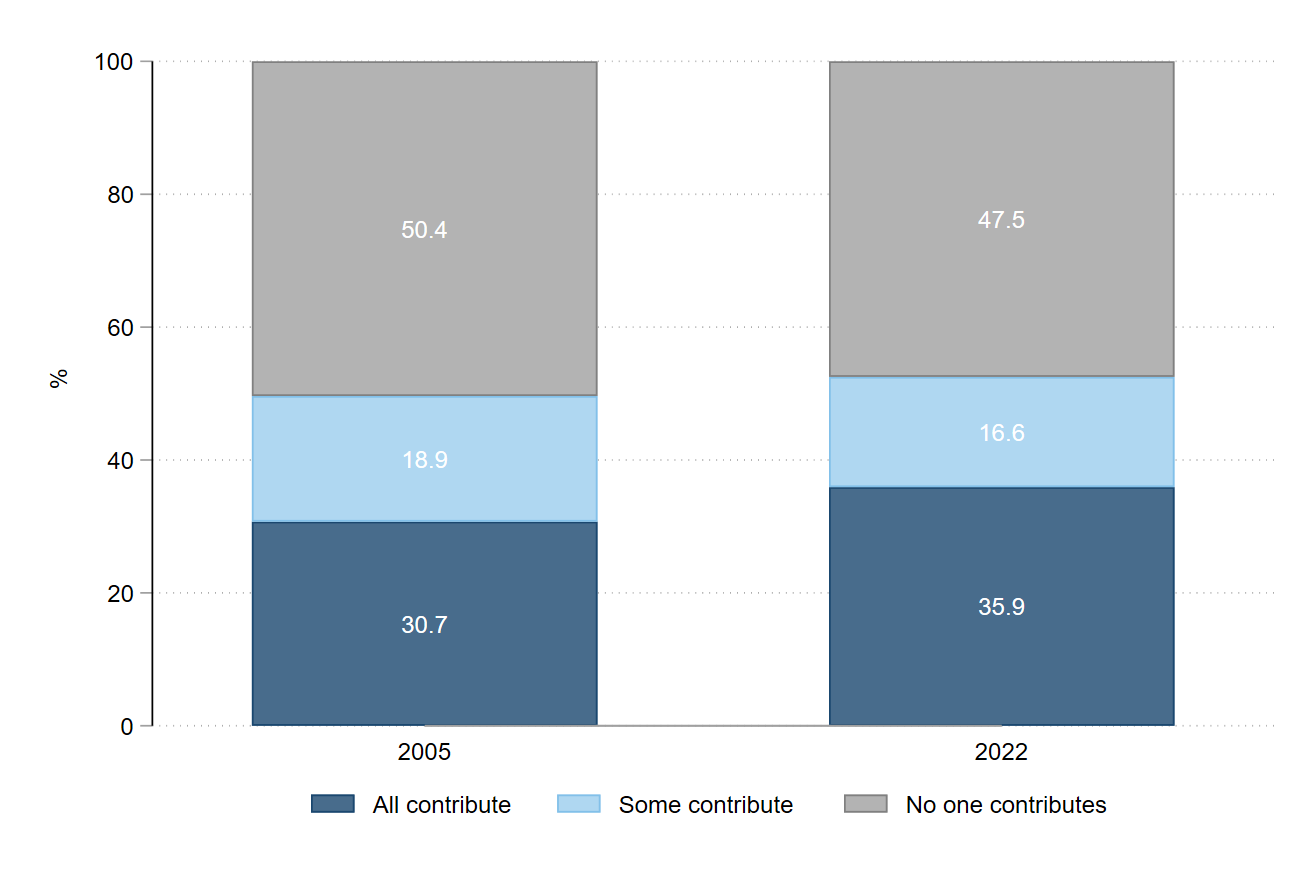
\includegraphics[scale=.3]{latex/figures/Household/snapshot_household_2005-2022_LAC}
    \label{fig:HouseholdLAC}}
    \footnotesize{Source: Household Surveys-SEDLAC.}
    \footnotesize{Note: Each bar is a weighted average of each country, weighting by total workers in 2005 and 2022. For countries without information for 2022 in SEDLAC we use the last available year: Bolivia 2021; Guatemala 2014; Honduras 2019 and Panama 2021.}
     \footnotesize{Note: The figure reports the household contribution status to social security of households with at least one member works. All contribute: corresponds to the percentage of households where all workers contribute to SS. Some contribute: corresponds to the percentage of households where some workers contribute to SS but not all. No one contributes: corresponds to the percentage of households where no workers contributes to SS.}
\end{figure}

\begin{landscape}
\begin{figure}[!htb]
    \centering
    \caption{Snapshot of LAC’s countries household employment condition for 2005-2022}     
    \centerline{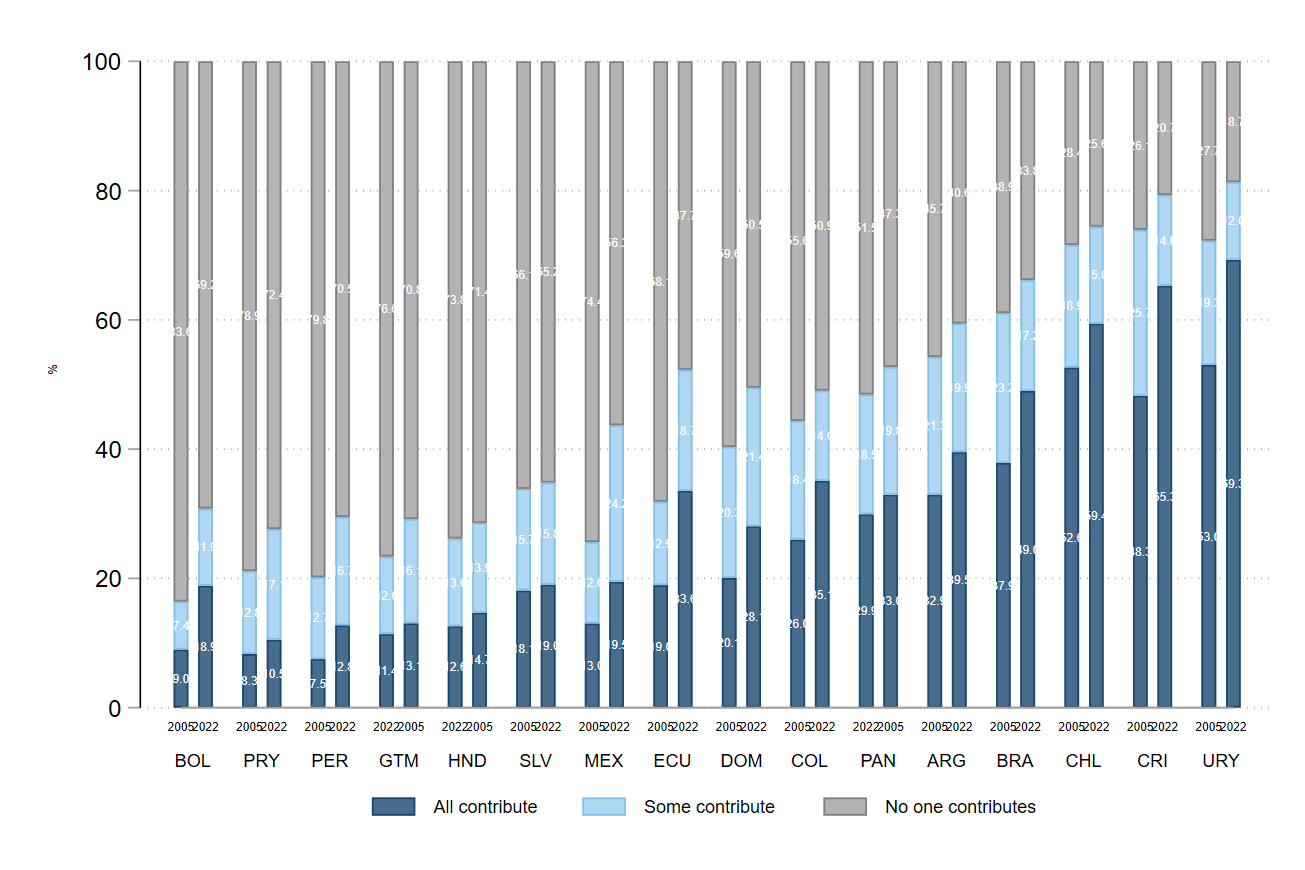
\includegraphics[scale=.45]{latex/figures/Household/snapshot_household_2005-2022.png}
    \label{fig:Household20052022}}
    \justifying
    \footnotesize{Source: Household Surveys-SEDLAC.}
    \footnotesize{Note: Each bar is a weighted average of each country, weighting by total workers in 2005 and 2022. For countries without information for 2022 in SEDLAC we use the last available year: Bolivia 2021; Guatemala 2014; Honduras 2019 and Panama 2021.}
    \footnotesize{Note: The figure reports the household contribution status to social security of households with at least one member works. All contribute: corresponds to the percentage of households where all workers contribute to SS. Some contribute: corresponds to the percentage of households where some workers contribute to SS but not all. No one contributes: corresponds to the percentage of households where no workers contributes to SS.}
\end{figure}
\end{landscape}

\subsubsection{Workers level} 
\begin{figure}[H]
    \justifying
     \caption{Workers who do not contribute to SS}     
     \centerline{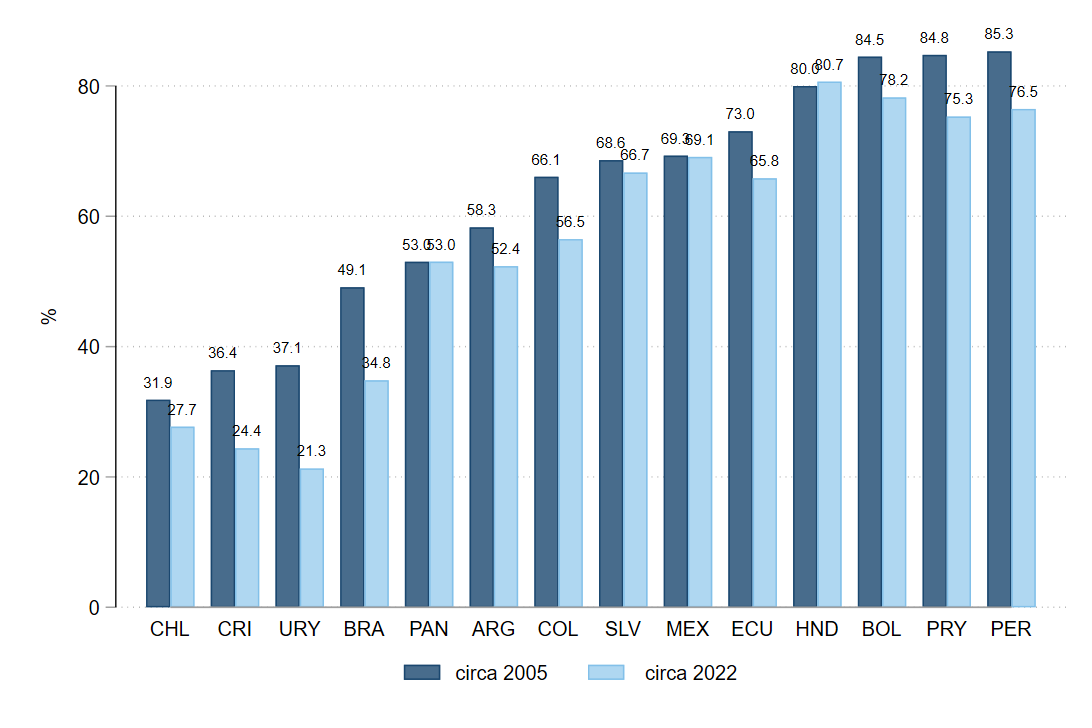
\includegraphics[scale=.3]{latex/figures/Snapshot/snapshot_informal_ss.png}
    \label{fig:SalariedSS}}
    \footnotesize{Source: Household Surveys-SEDLAC.}
    \footnotesize{Note: Each bar is a weighted average of each country, weighting by total workers in 2005 and 2022. For countries without information for 2022 in SEDLAC we use the last available year: Bolivia 2021; Guatemala 2014; Honduras 2019 and Panama 2021.}
\end{figure}

\begin{figure}[H]
    \justifying
     \caption{Salaried who do not contribute to SS}     
     \centerline{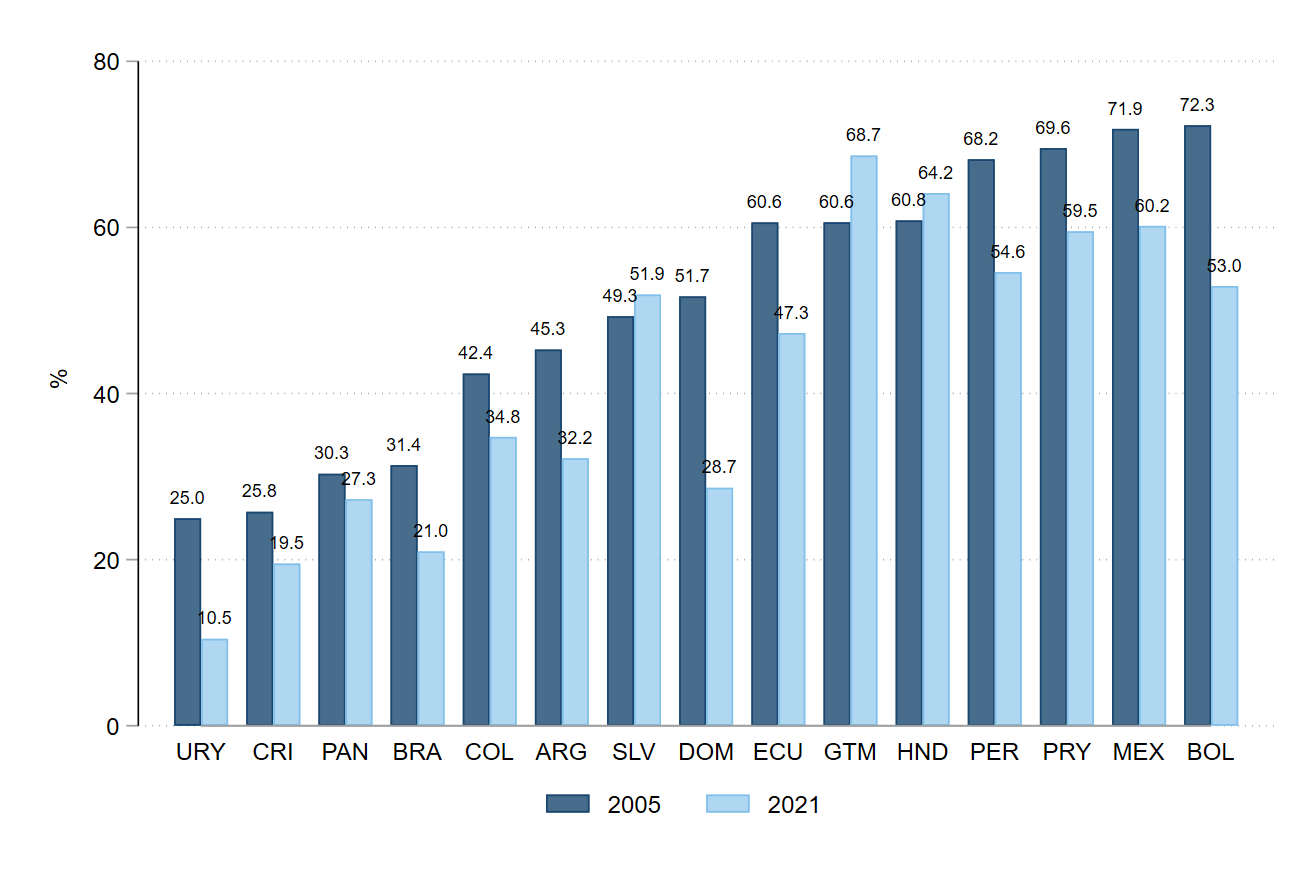
\includegraphics[scale=.3]{latex/figures/Snapshot/snapshot_informal_ss_dep.png}
    \label{fig:SalariedSS}}
    \footnotesize{Source: Household Surveys-SEDLAC.}
    \footnotesize{Note: Each bar is a weighted average of each country, weighting by total workers in 2005 and 2022. For countries without information for 2022 in SEDLAC we use the last available year: Bolivia 2021; Guatemala 2014; Honduras 2019 and Panama 2021.}
\end{figure}

\begin{figure}[H]
    \justifying
     \caption{Salaried who work at small firms}     
     \centerline{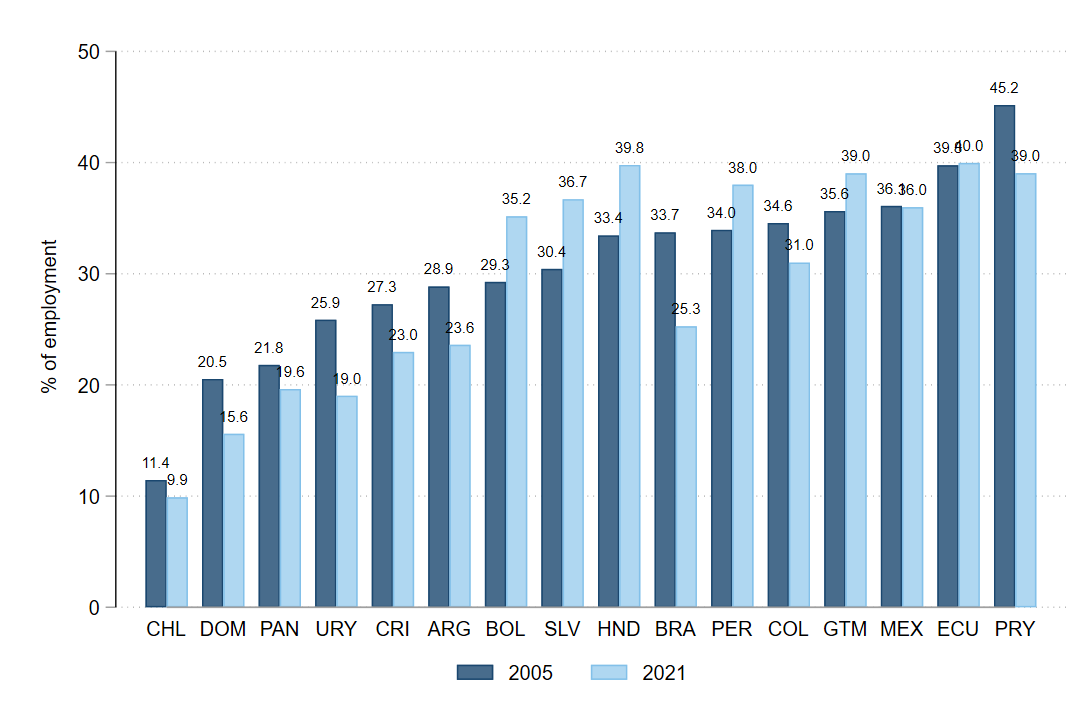
\includegraphics[scale=.3]{latex/figures/Snapshot/snapshot_dependents_small.png}
    \label{fig:SalariedSmall}}
    \footnotesize{Source: Household Surveys-SEDLAC.}
    \footnotesize{Note: Each bar is a weighted average of each country, weighting by total workers in small firms in 2005 and 2022. For countries without information for 2022 in SEDLAC we use the last available year: Bolivia 2021; Guatemala 2014; Honduras 2019 and Panama 2021.}
\end{figure}


\begin{figure}[H]
        \justifying
        \caption{Microeconometric decomposition of evolution of workers who does not contribute to ss 2005-2022}     
       \centerline{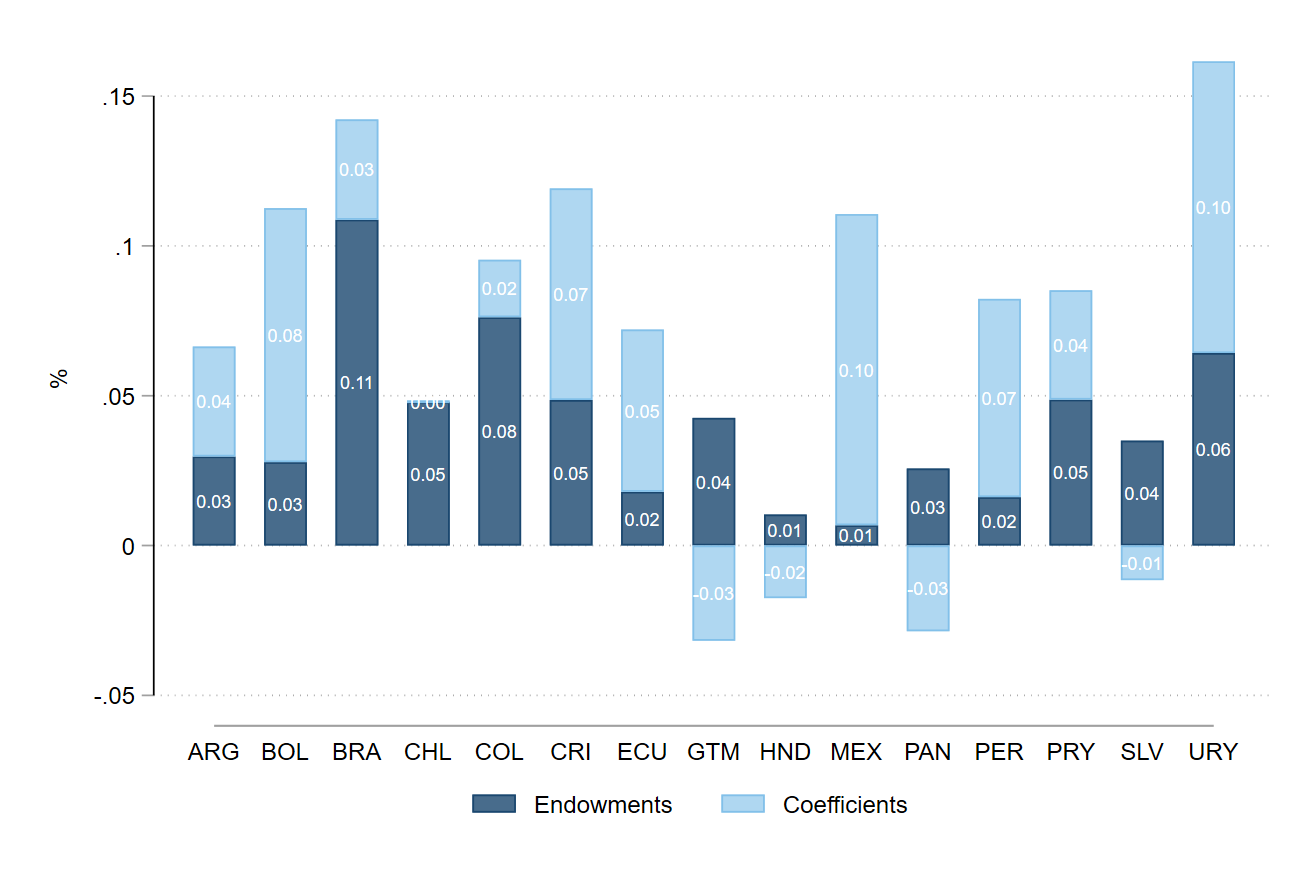
\includegraphics[scale=.3]{latex/figures/Snapshot/Oaxaca decomposition level.png}
        \label{fig:Oaxaca_level}}
        \footnotesize{Source: Household Surveys-SEDLAC.}
        \footnotesize{Note: Each bar is the actual change in Social security contributions corresponds to the level of coefficients and the level of the endowment effects.  Data corresponds to 2022. For countries without information for 2022 in SEDLAC we use the last available year: Bolivia 2021; Guatemala 2014; Honduras 2019 and Panama 2021.}
 \end{figure}


\newpage
\section{Appendix}
\subsection{Oaxaca methodology decomposition}
In order to determine the extent to which the change in the formality rate among wage earners in each country being studied is due to variations in the composition of employment (composition effect) and to what extent it is due to the formality rate of each group of workers (coefficient effect), an "aggregate" decomposition was calculated as a first step, as follows:

${\Delta}LF=\sum_{g=1}^{G}w_g^{0}.{\Delta}LF_g+\sum_{g=1}^{G}LF_g^{0}.{\Delta}w_g$

where:
\begin{itemize}

\item ${\Delta}LF$:change in labour formality rate between $t=1$ and $t=0$ 
\item ${\Delta}LF_g$:change in labour formality rate between $t=1$ and $t=0$ in subgroup g
\item ${\Delta}LF_g^{0}$:Labour formality rate of subgroup g in $t=0$
\item $w_g^{0}$:participation rate of group g in total wage earnerns in $t=0$
\item ${\Delta}w_g$:change in participation rate of group g in total wage earners between $t=1$ and $t=0$ 
\end{itemize}

The first term in the equation reflects the coefficient effect, which is the weighted sum of the changes in the formality rate of each of the various subgroups, where the weighted factor is the initial weight of each subgroup in total wage-earning employment. The second term reflects the composition effect, which results from the weighted sum of the changes in occupational structure, where the weighted factor is the initial specific formality rate of each group.
This exercise will be carried out separately for the dimensions of greatest significance for the structure of wage-earning employment in the countries concerned: branch of activity, size of enterprise, educational level and age.





\end{document}